%{\huge {\bf Local Information}}
\phantomsection
\addcontentsline{toc}{section}{Local Information}
\section*{Local Information}
%
%
\phantomsection
\addcontentsline{toc}{subsection}{Location}
\subsection*{Location}
\mlss, Sydney, 2015 will be held on the The Camperdown and Darlington Campuses at the University of Sydney. 
This 72-hectare site is located near the junction of Parramatta and City Roads just outside of downtown Sydney. It features landscaped grounds, sports ovals and centres, museums, galleries, two major complexes devoted to student recreation and services, and the famous Quadrangle and many other beautiful modern and historic buildings.  
%
\subsubsection*{Venues}
The following campus map shows the location of the  technical  and  practical (lab) sessions. \\ 
%
\underline{Technical Sessions:}
%
Bosch Lecture Theatre 2, Bosch building 1A,  map grid reference E7. \\
%
\underline{Practical Sessions:}
PNR Learning Studios 310, 311 and 315, Peter Nicol Russell (PNR) building, map grid reference N8.
%
%
%\clearpage
%\thispagestyle{empty}
%~\clearpage
%
\begin{figure}[h!]
%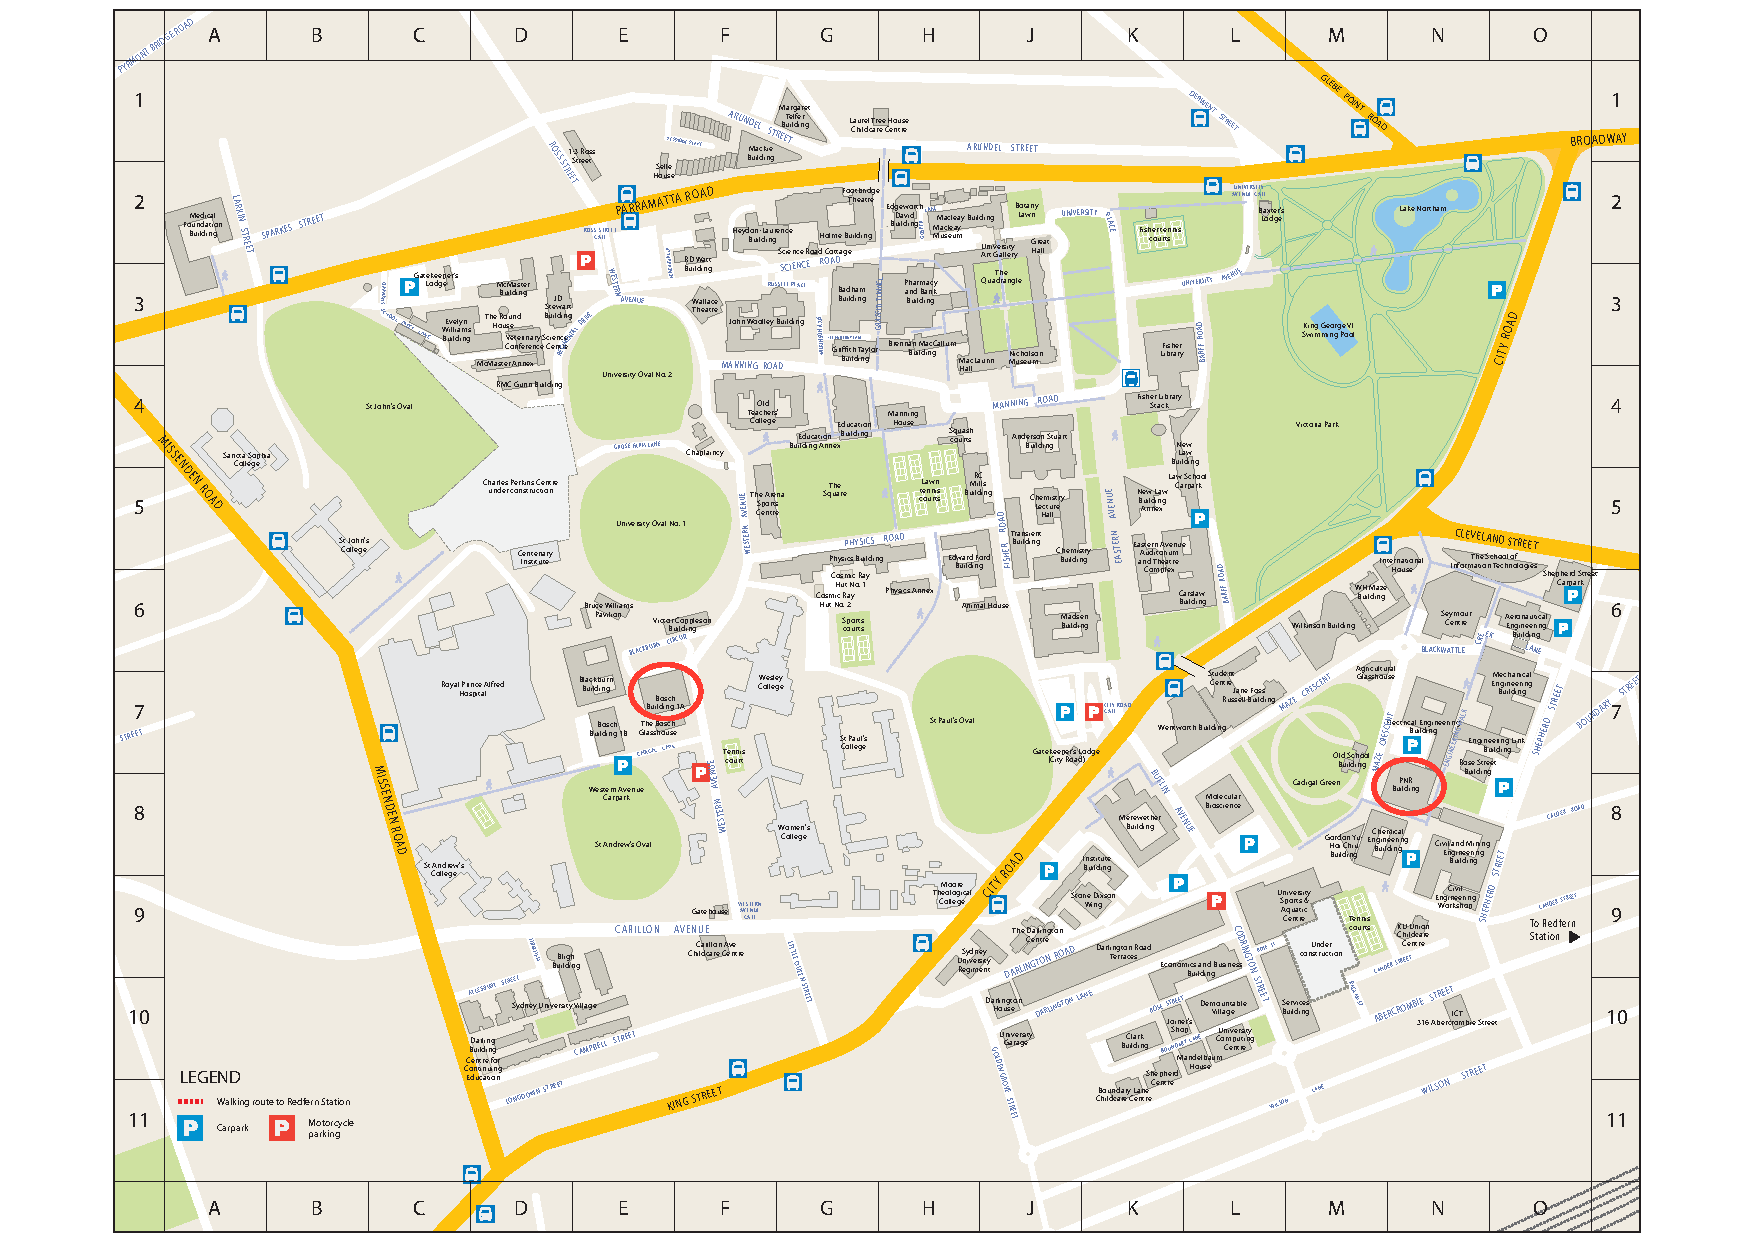
\includegraphics[width=\linewidth]{campus2}
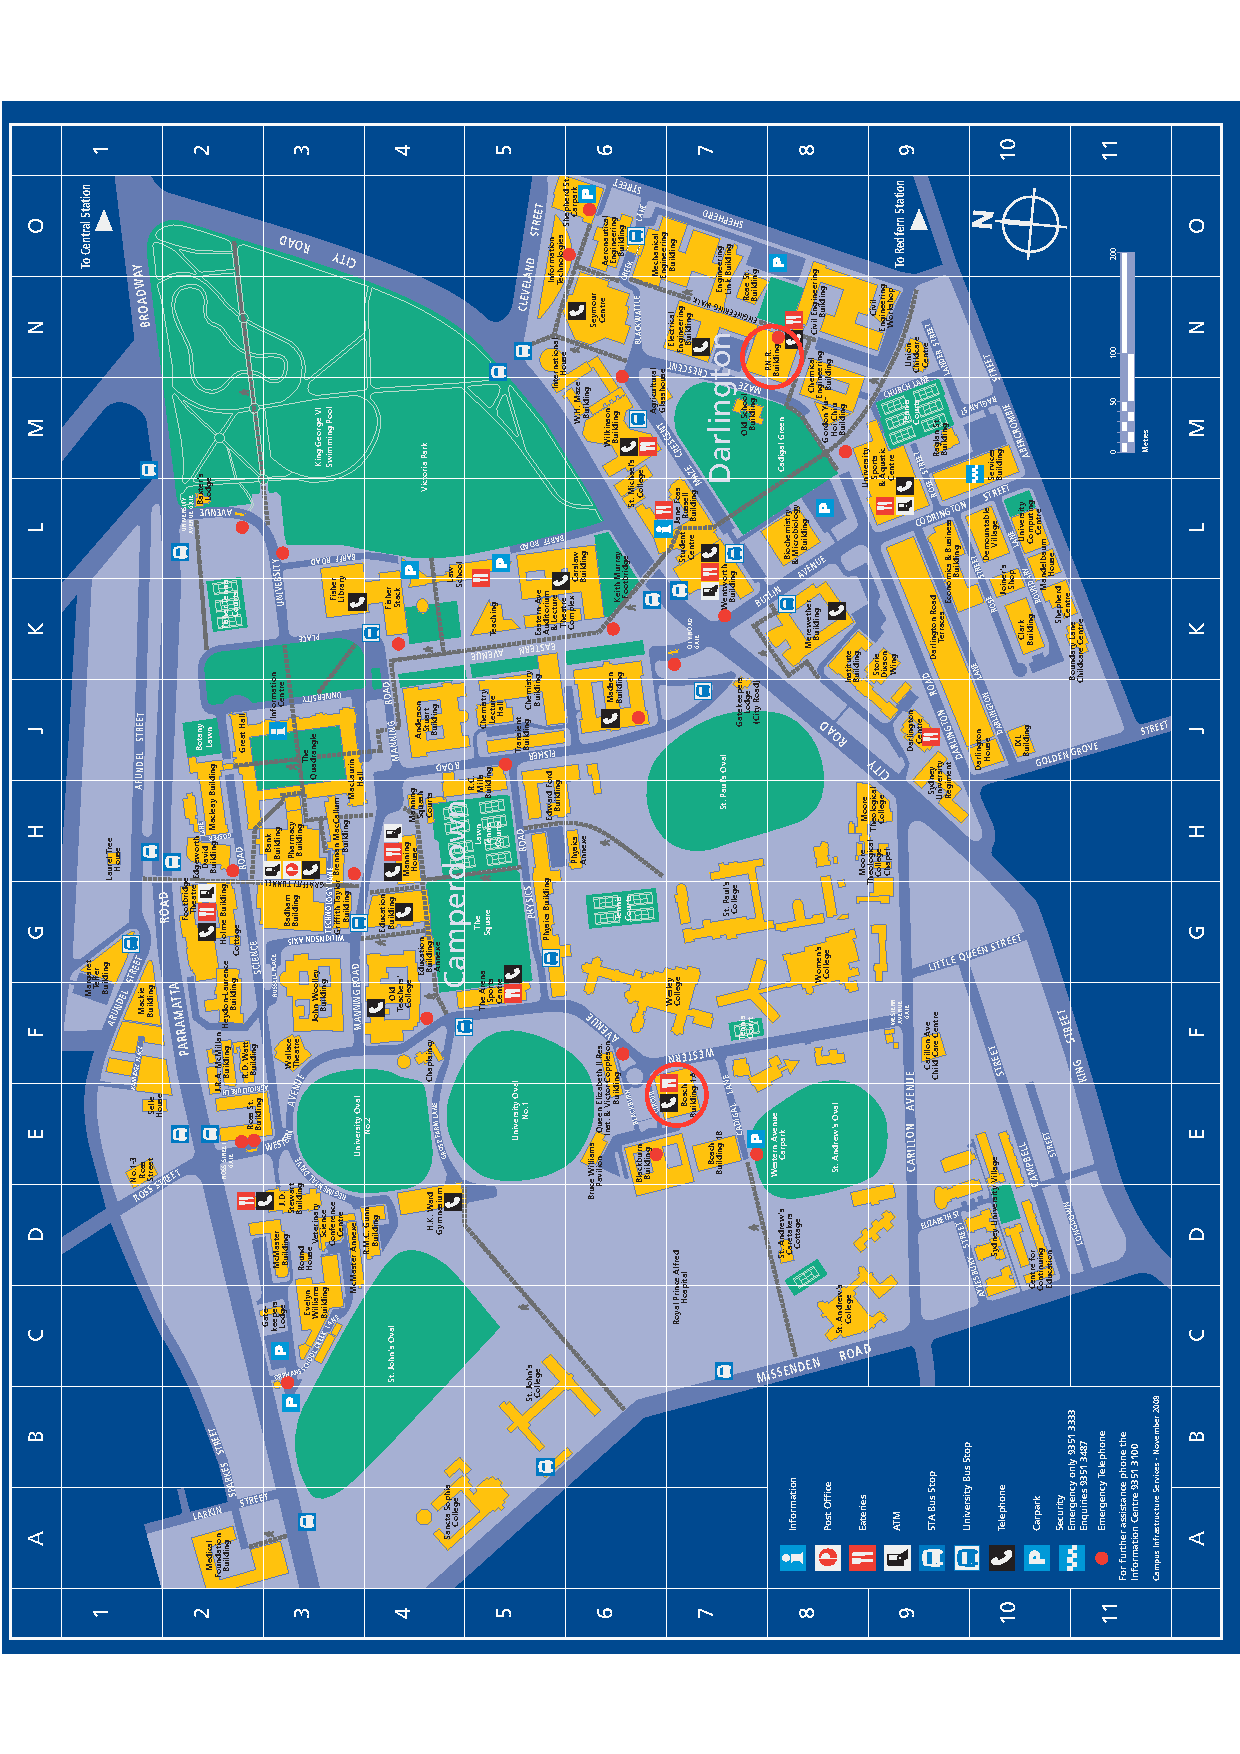
\includegraphics[width=\linewidth]{campus7}
\end{figure}

\clearpage


%\subsubsection*{About} 
%The University of Sydney is one of Australia’s leading research institutions. The country’s first tertiary education institution, it attracts some of the best students, researchers and academic staff from around the world. It is unique among Australian universities in the breadth of disciplines on offer, providing wide opportunities for personal development and cross-disciplinary study that delivers unique insights and breakthroughs.
%Since its foundation in 1850, the University has produced over 270,000 graduates – many who lead their fields both nationally and on the world stage. The University can proudly claim four Prime Ministers, an early president of the United Nations, two Governors-General, two Nobel Laureates, several Chief Justices and High Court Judges, presidents of the Royal Society and World Bank, business leaders, outstanding literary writers, poets and an Oscar-winning film director.
\phantomsection
\addcontentsline{toc}{subsection}{Getting There}
\subsection*{Getting There}
\begin{itemize}
 \item By train: Catch a train to Redfern train station, and then take a 10-minute walk to the main campus. Timetables, network information and route planners are available from the City Rail website.
\item By bus from the City: For stops on Parramatta Road (closest to the Quadrangle) catch routes 412, 413, 435, 436, 437, 438, 440, 461, 480 and M10 from George Street or Railway Square.
For stops on City Road (closest to Darlington Campus) catch routes 422, 423, 426, 428 from Castlereagh Street or Railway Square.
\item By bus - cross routes: Route 370 runs between Coogee and Leichhardt. 
Route 352 runs between Bondi Junction and Marrickville.
Route M30 runs between Mosman, George St in the city and Sydenham. Alight on City Rd for Sydney University.
\item By Taxi: The University is readily accessible by taxi from the airport (approx. 20 minutes) and the city (also a 20 minute fare).
\end{itemize}
%
\phantomsection
\addcontentsline{toc}{subsection}{Accommodation}
\subsection*{Accommodation}
There are a variety of accommodation options available in Sydney. Accommodation close to the \mlss 2015 venue is available
at a number of hotels near the campus or in the city that are readily accessible. 
There are also many Budget accommodation options around the campus and in the city. A number of online booking services provide discounted rates for hotels in Sydney. Buses and trains provide ready access to the University of Sydney campus from most areas of the city. See \url{http://nicta.com.au/research/machine_learning/mlss2015/mlss-accommodation} for details.
%
\phantomsection
\addcontentsline{toc}{subsection}{Registration}
\subsection*{Registration}
The Summer School is not a commercial activity and all the money collected from registrations and sponsorships is used for the expenses 
of the school. For all attendees registration includes admission to all MLSS 2015 main technical sessions
and lab sessions, coffee breaks, and lunches for the working days, 
as well as attendance to the banquet. 
The registration fee does not include dinners, breakfasts or accommodation. 
%
%
\newpage
\phantomsection
\addcontentsline{toc}{subsection}{Organisers and Sponsors}
\phantomsection
\subsection*{Organisers and Sponsors}
NICTA, The University of Sydney, and The University of New South Wales are the 
organisers of MLSS Sydney 2015.
%
\subsubsection*{Organized by}
\begin{center}

\includegraphics[height=1in]{nicta-logo-small}

\includegraphics[height=1in]{usydney-logo}

\includegraphics[height=0.8in]{unsw-logo}
\end{center}
%
\subsubsection*{Financial sponsors}
MLSS gratefully acknowledges the following sponsors.  In
addition to other benefits, sponsor support allows the school to
keep its registration  fees to a minimum, particularly for
students.
%
%\begin{center}
%{\fontfamily{cmr}\selectfont {\LARGE PLATINUM SPONSOR}}
%\end{center}
 \vspace{-0.2in}
\begin{center}
  \begin{figure*}[h!]
\centering
     
\includegraphics[height=1in]{nicta-logo}
     \includegraphics[height=1in]{cba-logo}     
 
\includegraphics[height=1in]{usydney-logo}
    \end{figure*}
\end{center}
%
\phantomsection
\addcontentsline{toc}{subsection}{Coffee Breaks and Lunch}
\subsection*{Coffee Breaks and Lunch}
\mlss will provide coffee and tea for each of the main technical sessions 
 and lunch for every working day. These will take place at the same location as 
 the main technical sessions (Bosch Building 1A).
%
%
%
\phantomsection
\addcontentsline{toc}{subsection}{Banquet}
\subsection*{Banquet}  
%
We will get together for dinner and drinks on Tuesday 24th February from 7pm-10pm , all while cruising  the beautiful 
surroundings of Sydney Harbour.

\underline{Meet up Location}:  \\
Starship Sydney \& The Pontoon \\ 
King Street Wharf 4, Sydney \\
 \url{https://goo.gl/maps/OSp3k}.
%
\phantomsection
\addcontentsline{toc}{subsection}{Nearby Restaurants}
\subsection*{Nearby Restaurants}
For food and drinks around the University of Sydney please see: \\
- \url{http://www.seymourcentre.com/local-restaurants}; and \\ 
- \url{http://sydney.edu.au/current_students/life/food.shtml}.


%\subsubsection*{Restaurants}
%\adnote{add restaurants}
%
%
%\subsubsection*{Pubs}
%\adnote{add Pubs}
%
%\subsubsection*{Cocktail Bars (From Sydney's Best Bar Awards 2012)}
%\begin{itemize}
% \item Victoria Room: ``The Victoria Room is the real deal, combining craft cocktails, incredible bartender knowledge and a beautiful venue.''
%\item Eau de Vie: ``This speakeasy-style bar has a wealth of talented bartenders working with exceptional hooch. It’s an industry haunt, a den of iniquity, and probably the best fun you can have with a glass in your hand.''
%\item Low 302: ``The Crown Street stalwart has been delivering on the cocktail front since ’09 and they’re showing no signs of slowing down. You might go for a beer (and many do) but you’d be mad not to stay for a Gimlet.''
%\item Rockpool Bar and Grill: ``If there’s one place in Sydney you’re guaranteed to get a great drink and a great snack, it’s here. Bartenders make their own sodas and syrups and can rustle up a tasty drink faster than you can say Julep''
%\item Shady Pines: ``They’ll pour you a beer as fast as they pour a Sazerac and all with the same level of attention and care. If you haven’t had them make you a Negroni topped with Coke (blasphemous!) then you haven’t truly lived.''
%\end{itemize}

\phantomsection
\addcontentsline{toc}{subsection}{What to Do}
\subsection*{What to Do}
Within easy access of the University:
\begin{itemize}
 \item Aquarium
\item Wildlife World (see some kangaroos and wallabies!!)
\item Opera House
\item Bridge climb
\item Ferry to Manly Beach
\item Coogee Beach
\item Bondi Beach
\end{itemize}

Further afield:
\begin{itemize}
 \item Hunter Valley (great wine)
\item The Blue Mountains (stunning scenery)
\item Jervis Bay (South) and Nelson Bay (North) (see some dolphins!!)
\item The Great Barrier Reef is a half day flight away
\item Uluru (a large sandstone rock formation in central Australia) 
\end{itemize}

% \subsection*{Location}
% 
% The conference will be held on the campus of the University of
% Southern California (USC) in Los Angeles, California, USA. USC is
% located close to Los Angeles downtown, which is home to a high density
% of cultural and social hotspots, including many restaurants and
% bars. The main conference will be held in the Andrus Gerontology
% Auditorium (GER) on the USC campus. This is also the site for all
% sponsor displays. Workshops will be held in the Grace Ford Salvatori
% Hall (GFS) on the USC campus. The interactive poster session will be
% held in the ballroom of the Radisson Hotel (RMH). The map below shows
% the USC campus with the main conference site and workshop locations as
% well as the two recommended housing choices.
% 
% \bigskip
% \begin{center}
% \includegraphics[width=1.0\columnwidth]{local_img/usc_map.png} 
% \\
% \includegraphics[width=1.3\columnwidth, angle=90]{local_img/map.png} 
% \end{center}
% 
% \clearpage
% \section*{Registration}
% 
% The Conference Desk will be staffed for registration and information
% services according to the following schedule:
% 
% \bigskip
% \bigskip
% \begin{tabular}{ l l }
%  Monday, June 27  & 8:30 to 16:00 (at the Grace Ford Salvatori Hall (GFS))  \\
%  Tuesday, June 28 & 8:30 to 17:00 (at the Andrus Gerontology Auditorium (GER))   \\
%  Wednesday, June 29  & 8:30 to 13:00 (at the Andrus Gerontology Auditorium (GER)) \\
%  Thursday, June 30  & 8:30 to 13:00 (at the Andrus Gerontology Auditorium (GER))  \\
%  Friday, July 1  & 8:30 to 13:00 (at the Grace Ford Salvatori Hall (GFS)) \\
% \end{tabular}
% 
% \bigskip
% \bigskip
% The conference registration fees are:
% \bigskip
% \begin{center}
% \begin{tabular}{ l c c| c c }
% & \multicolumn{2}{c|}{Early (until June 1)} &  \multicolumn{2}{c}{Regular (after June 1)}   \\ [3pt]
%  \cline{2-5} 
% &  Student & Non-Student & Student & Non-Student\\ [3pt]
%  Regular:  &  \$225 & \$450 & \$300 & \$550  \\
% June 27 workshop-only:  &  \$100 & \$150  & \$150 & \$250\\
% July 1 workshop-only:  &   \$100 & \$150  & \$150 & \$250\\
%  Both workshop days:  &  \$200 & \$300  & \$300 & \$500 \\
% \end{tabular}
% \end{center}
% \bigskip
% Both student and non-student registration includes attendance to the
% main conference oral and poster sessions, as well as the workshops on
% Monday, June 27th and Friday, July 1st. In addition, it includes one
% hardcopy of the conference proceedings, and one ticket for the
% conference banquet on Wednesday, June 29th evening at {\it Spago} in
% Beverly Hills.
% \bigskip
% \\
% A workshop registration for one day includes access to any of the
% workshops on that day. It does {\bf not} include access to the
% conference proper, a hardcopy of the proceedings, and the banquet.
% \bigskip
% \\
% A workshop registration for two days includes access to all
% workshops. It does {\bf not} include access to the conference proper,
% a hardcopy of the proceedings, and the banquet.
% \bigskip
% \\
% At registration, attendees may purchase extra banquet tickets
% (e.g. for companions). Each extra banquet ticket is \$175.
% \bigskip
% \\
% The registration desk at the conference accepts only major credit
% cards. No cash or check transactions are possible.
% 
% \newpage
% 
% \clearpage
% \section*{Sponsors}
% The conference gratefully acknowledges the following sponsors.  In
% addition to other benefits, sponsor support allows the conference to
% keep its registration and workshop fees to a minimum, particularly for
% students.
% 
% \bigskip
% \bigskip
% {\bf \underline{Financial sponsors:}}
% 
% \begin{center}
% {\fontfamily{cmr}\selectfont {\LARGE GOLD SPONSORS}}
% \end{center}
%  \vspace{-0.2in}
% \begin{center}
%   \begin{table*}[h!]
%     \begin{tabular}{ >{\centering} p{0.5\textwidth}   >{\centering}p{0.45\textwidth} }
%      \includegraphics[width=2.0in]{local_img/Google_Logo_292X94.png} & \includegraphics[width=1.2in]{local_img/WG_logo_on_black.pdf} 
%     \end{tabular}
%   \end{table*}
% \end{center}
% \begin{center}
% \vspace{-0.4in}
% {\fontfamily{cmr}\selectfont {\Large SILVER SPONSORS}}
% \end{center}
% \vspace{-0.2in}
% \begin{center}
%   \begin{table*}[h!]
%     \begin{tabular}{ >{\centering} p{0.5\textwidth}   >{\centering}p{0.45\textwidth} }
%      \includegraphics[width=2.0in]{local_img/mslogo.jpg} & \includegraphics[width=1.8in]{local_img/irobot.jpg} 
%     \end{tabular}
%   \end{table*}
% \end{center}
% \begin{center}
% \vspace{-0.4in}
% {\fontfamily{cmr}\selectfont {\large BRONZE SPONSORS}}
% \end{center}
% \vspace{-0.2in}
% \begin{center}
%   \begin{table*}[h!]
%     \begin{tabular}{ >{\centering} p{0.5\textwidth}   >{\centering}p{0.45\textwidth} }
%      \includegraphics[width=2.0in]{local_img/Barrett_Technology_Logo_2010.png} & \includegraphics[width=2.0in]{local_img/Aldebaran.png} 
%     \end{tabular}
%   \end{table*}
%   \vspace{-0.6in}
% \end{center}
% \begin{center}
%   \begin{table*}[h!]
%     \begin{tabular}{ >{\centering} p{0.5\textwidth}   >{\centering}p{0.45\textwidth} }
%      \includegraphics[width=2.0in]{local_img/lockheed.png} & \includegraphics[width=2.0in]{local_img/abb_logo.png} 
%     \end{tabular}
%   \end{table*}
% \end{center}
% \vspace{-0.3in}
% {\bf \underline{Award Sponsors:}}
% \vspace{-0.2in}
% \begin{center}
%   \begin{table*}[h!]
%     \begin{tabular}{ >{\centering} p{0.3\textwidth}   >{\centering}p{0.3\textwidth} >{\centering}p{0.3\textwidth} }
%      \includegraphics[width=1.5in]{local_img/irobot.jpg} & \includegraphics[width=1.5in]{local_img/Google_Logo_292X94.png} & \includegraphics[width=1.5in]{local_img/Springer_Media_fc_logo_full.jpg} 
%     \end{tabular}
%   \end{table*}
% \end{center}
% \begin{center}
% \vspace{-0.1in}
%   \begin{table*}[h!]
%     \begin{tabular}{ >{\centering} p{0.3\textwidth}   >{\centering}p{0.3\textwidth} >{\centering}p{0.3\textwidth} }
%     \vspace{-0.5in} {\bf Best Paper Award} & \vspace{-0.5in}{\bf Travel Awards} & \vspace{-0.5in}{\bf Best Student Paper Award}
%     \end{tabular}
%   \end{table*}
% \end{center}
% \vspace{-0.6in}
% {\bf \underline{Technical Sponsors:}}
% \vspace{-0.1in}
% %The 2011 Robotics: Science and Systems conference is furthermore supported by the following technical sponsors:
% 
% \begin{center}
% \includegraphics[width=0.7in]{local_img/RAS_logo_2c.jpg}
% \includegraphics[width=2.0in]{local_img/IEEE_logo.png}
% \includegraphics[width=0.9in]{local_img/aaai_logo.png}
% \includegraphics[width=0.6in]{local_img/IFRR.png}
% \end{center}
% 
% {\bf \underline{Organized by:}}
%  \vspace{-0.0in}
% \begin{center}
% \includegraphics[width=0.6in]{local_img/seal_card_trans.pdf}
% \includegraphics[width=2.0in]{local_img/12462.pdf}
% \end{center}
% 
% \bigskip
% \bigskip
% \newpage
% 
% \section*{Workshop Locations}
% 
% The workshops on Both {\bf Monday, June 27th} and {\bf Friday, July 1st} will take place in the \\
% \underline{Grace Ford Salvatori Hall (GFS)} on the USC Campus.
% %{\bf Monday, June 27th} workshop will take place in the \underline{Grace Ford Salvatori Hall (GFS)} on the USC Campus.
% \bigskip
% \\
%  {\bf Monday, June 27th} workshops
%  
% \begin{itemize}
% 
% \item  {\bf WS1. RGB-D: Advanced Reasoning with Depth Cameras}\\
% 	\textit{Location: GFS 101}  \\
% \begin{tabular}{ l l }
% \hspace{-2mm}\textit{Organizers: } &  Dieter Fox, University of Washington \\
% &  Kurt Konolige, Willow Garage \\
% &  Jana Kosecka, George Mason University \\
% & Xiaofeng Ren,	Intel Labs Seattle
% \end{tabular}
% 
% \item  {\bf WS2. The State of Imitation Learning: Understanding its Applications and Promoting its Adoption}\\
% 	\textit{Location: GFS 201}  \\
% \begin{tabular}{ l l }
% \hspace{-2mm}\textit{Organizers: } &  Brenna Argall, \'{E}cole Polytechnique F\'{e}d\'{e}rale de Lausanne EPFL \\
% &  Nathan Ratliff, Google \\
% &  David Silver, Carnegie Mellon University
% \end{tabular}
% 
% \item  {\bf WS3. Toward High-Performance Computing Support for the Analysis, Simulation, and Planning of Robotic Contact Tasks}\\
% 	\textit{Location: GFS 202 $\&$ GFS 101 (June 28th morning)}  \\
% \begin{tabular}{ l l }
% \hspace{-2mm}\textit{Organizers: } &  Chris Carothers, Rensselaer Polytechnic Institute \\
% &  Dan Negrut, University of Wisconsin \\
% &  Jeff Trinkle, Rensselaer Polytechnic Institute
% \end{tabular}
% 
% \item  {\bf WS5. ALONE - Autonomous Long-Term Operation in Novel Environments}\\
% 	\textit{Location: GFS 104}  \\
% \begin{tabular}{ l l }
% \hspace{-2mm}\textit{Organizers: } &  Jonathan Kelly, University of Southern California \\
% &  Paul Newman, University of Oxford \\
% &  Sebastian Thrun, Stanford University / Google
% \end{tabular}
% 
% \item  {\bf WS6. Aquatic Robotics: Ocean Science and Marine Systems}\\
% 	\textit{Location: GFS 105}  \\
% \begin{tabular}{ l l }
% \hspace{-2mm}\textit{Organizers: } &  Ryan N. Smith, Queensland University of Technology \\
% &  Noel Du Toit, California Institute of Technology \\
% &  Burton H. Jones, University of Southern California \\
% & Kanna Rajan, Monterey Bay Aquarium Research Institute
% \end{tabular}
% 
% \item  {\bf WS7. Guaranteeing Motion Safety for Robots}\\
% 	\textit{Location: GFS 109} \\
% \begin{tabular}{ l l }
% \hspace{-2mm}\textit{Organizers: } &  Thierry Fraichard, INRIA Grenoble Rhone-Alpe \\
% &  Kostas Bekris, University of Nevada \\
% &  Jur van den Berg, University of North Carolina 
% \end{tabular}
% 
% \item  {\bf WS8. Mobile Manipulation - Learning to Manipulate}\\
% 	\textit{Location: GFS 118} \\
% \begin{tabular}{ l l }
% \hspace{-2mm}\textit{Organizers: } &  Thierry Fraichard, INRIA Grenoble Rhone-Alpe \\
% &  Kostas Bekris, University of Nevada \\
% &  Jur van den Berg, University of North Carolina 
% \end{tabular}
% 
% \end{itemize}
% 
% %{\bf Friday, July 1st} workshop will take place in the \underline{Grace Ford Salvatori Hall (GFS)} on the USC Campus.
% \clearpage
% {\bf Friday, July 1st} workshops
% \begin{itemize}
% 
% \item  {\bf WS9. Tutorial on 3D Point Cloud Processing: Point Cloud Library}\\
% 	\textit{Location: GFS 116} \\
% \begin{tabular}{ l l }
% \hspace{-2mm}\textit{Organizers: } &  Radu Bogdan Rusu, Willow Garage \\
% &  Bastian Steder, University of Freiburg \\
% &  Nico Blodow, Technical University of Munich \\
% &  Dirk Holz, University of Bonn
% \end{tabular}
% 
% \item  {\bf WS10. A Comparison of Reinforcement Learning and Optimal Control Methods for Real-World Robotic Tasks}\\
% 	\textit{Location: GFS 107} \\
% \begin{tabular}{ l l }
% \hspace{-2mm}\textit{Organizers: } &  Freek Stulp, University of Southern California \\
% &  Evangelos Theodorou, University of Southern California \\
% &  Stefan Schaal, University of Southern California
% \end{tabular}
% 
% \item  {\bf WS11. Integrated Planning and Control}\\
% 	\textit{Location: GFS 118} \\
% \begin{tabular}{ l l }
% \hspace{-2mm}\textit{Organizers: } &  Surya Singh, ACFR, The University of Sydney \\
% &  Russ Tedrake, Robot Locomotion Group, MIT \\
% &  Peter Corke, CyPhy Lab, Queensland University of Technology 
% \end{tabular}
% 
% \item  {\bf WS12. Human-robot interaction: Perspectives and contributions to robotics from the human sciences}\\
% 	\textit{Location: GFS 101} \\
% \begin{tabular}{ l l }
% \hspace{-2mm}\textit{Organizers: } &  Leila Takayama, Willow Garage \\
% &  Maja Mataric, University of Southern California \\
% &  Odest Chadwicke Jenkins, Brown University \\
% & Holly Yanco, University of Massachusetts Lowell \\
% & Brian Scassellati, Yale University
% \end{tabular}
% 
% \item  {\bf WS13. Automated SLAM Evaluation}\\
% 	\textit{Location: GFS 104} \\
% \begin{tabular}{ l l }
% \hspace{-2mm}\textit{Organizers: } &  Michael Kaess, Massachusetts Institute of Technology \\
% &  Giorgio Grisetti, Sapienza University of Rome/University of Freiburg \\
% &  Kai Ni, Georgia Institute of Technology/Microsoft
% \end{tabular}
% 
% \item  {\bf WS14. Tutorial on Dynamic Vehicle Routing for Robotic Systems}\\
% 	\textit{Location: GFS 105} \\
% \begin{tabular}{ l l }
% \hspace{-2mm}\textit{Organizers: } &  Francesco Bullo, University of California, Santa Barbara \\
% &  Emilio Frazzoli, Massachusetts Institute of Technology \\
% &  Marco Pavone, NASA JPL, California Institute of Technology \\
% & Ketan Savla, Massachusetts Institute of Technology \\
% & Stephen L. Smith, University of Waterloo
% \end{tabular}
% 
% \item  {\bf WS15. 3D Exploration, Mapping, and Surveillance with Aerial Robots}\\
% 	\textit{Location: GFS 108} \\
% \begin{tabular}{ l l }
% \hspace{-2mm}\textit{Organizers: } & Nathan Michael, University of Pennsylvania \\
% &  Mac Schwager, University of Pennsylvania \\
% &  Vijay Kumar, University of Pennsylvania
% \end{tabular}
% 
% \item  {\bf WS16. Tutorial on Stochastic Models, Information Theory, and Lie Groups}\\
% 	\textit{Location: GFS 109} \\
% \begin{tabular}{ l l }
% \hspace{-2mm}\textit{Organizers: } & Gregory S. Chirikjian, Johns Hopkins University
% \end{tabular}
% 
% \clearpage
% 
% \item  {\bf WS17. HRI Workshop on Grounding Human-Robot Dialog for Spatial Tasks}\\
% 	\textit{Location: GFS 109} \\
% \begin{tabular}{ l l }
% \hspace{-2mm}\textit{Organizers: } & Thomas Kollar, Massachusetts Institute of Technology \\
% & Stefanie Tellex, Massachusetts Institute of Technology \\
% & Robert Ross, Dublin Institute of Technology \\
% & Antoine Raux, Honda Research Institute \\
% & Matthew Marge, Carnegie Mellon University
% \end{tabular}
% \end{itemize}
% 
% \section*{Exhibits}
% The current list of exhibitors includes:
% 
% \bigskip
% \begin{tabular}{l@{\hspace{1in}}l}
% $\bullet$ Willow Garage  &\\
% $\bullet$ Aldebaran Robotics&\\
% $\bullet$ Microsoft & \\
% $\bullet$ iRobot & \\
% $\bullet$ Barrett Technology&
% \end{tabular}
% \bigskip
% \\
% The exhibits will be displayed from Tuesday, June 28th to Thursday,
% June 30th in the Andrus Gerontology Courtyard (GER) courtyard on the
% USC Campus.
% 
% \section*{Poster Session and Buffet Lunch}
% 
% The poster session will take place on Wednesday, June 29th from 13:15
% to 16:30 in the ballroom of the Radisson Hotel (RMH).  The poster
% session will begin with a catered buffet lunch at the same location.
% \bigskip
% \\
% Unlike previous years, posters will be presented electronically on big
% screen displays. Poster presenters should bring their own laptop
% to display their poster. The conference will provide a power outlet for
% the laptop and a VGA cable to connect the laptop to the large LCD
% display. The display will be mounted in 'landscape' mode. Please make
% your poster accordingly.
% \bigskip
% \\
% Presenters may arrive at the Radisson ballroom anytime after 12:00 to test
% their laptop's connection to the display.
% 
% \section*{Banquet}
% 
% The conference banquet will be held on Wednesday, June 29th at {\it
% Spago} located in Beverly Hills. Buses for the banquet will leave from
% the Radisson hotel at 17:00. After the banquet the buses will return
% attendees to the Radisson. This excursion is complimentary with full
% conference registration. Each registrant will receive a banquet ticket
% with the registration packet. Each registrant should make sure you to
% have the banquet ticket handy when boarding the bus.  Additional
% banquet tickets may be purchased for \$175 per person. The banquet
% will commence with a cocktail reception featuring an unusual
% appetizer: a robot-related video session designed to provoke, amuse
% and entertain.
% 
% \section*{USC Robotics Lab Tours}
% 
% The robotics labs at USC will hold an open house in the lunch break on
% Tuesday June 28th (from 13:15 to 14:30). This is not a catered lunch
% event. Conference attendees are encouraged to pick up a quick lunch
% from one of the on-campus eateries and come to the 4th floor of Ronald
% Tutor Hall (RTH) [across the street from the Geontology Center (GER)]
% to see short displays and presentations by USC students about their
% research.
% 
% \clearpage
% 
% \section*{Accommodation}
% 
% The following accommodation options are available. Keeping in mind
% that hotels in the Los Angeles area are expensive and one typically
% needs a car to get around, the conference organizers have tried to
% make affordable housing arrangements within walking distance of the
% conference site. It is strongly recommended that attendees use one of
% the two options below.
% \begin{itemize}
% \item  Student dorms:  \\
%  Shared bedroom, shared bath: \$38 \\
%  Private bedroom, shared bath: \$50 \\
% USC Parkside International Residential College (IRC)\\
% 3771 S McClintock Avenue\\
% Los Angeles, CA 90007 \\
% 
% Check-in at Parkside is available at the Parkside complex itself.
% Parkside residents will receive the access cards for their rooms upon
% checking in. The USC campus is open 24 hours. The entry gate number 6
% (located on Vermont and 36th Place) is open round the clock for campus
% access. For late check-in or check-out (or if you are locked out of
% your room) please call (213) 986-6USC.
% 
% \item USC Radisson Hotel: \$139\\
% 3540 South Figueroa Street \\
% Los Angeles, CA 90007 \\
% phone: (213) 748-4141
% \end{itemize}
% 
% Both recommended conference accommodations are at walking distance
% (maximum 10 minutes) to the conference site.
% 
% \section*{Internet Access}
% Wireless internet access will be available at the conference site via
% USC Wireless. The system is open to guest users. No password is needed.
% 
% \section*{Lunch Breaks}
% 
% As part of the conference registration, lunch will be provided on
% Wednesday June 29 (buffet lunch as part of the poster session) and
% Thursday June 30 (box lunch for the open sessions).  There will be
% morning and afternoon coffee breaks with snacks every day during the
% workshops and the main conference.
% \bigskip
% \\
% On the workshop days and on Tuesday June 28, all attendees are
% encouraged to plan accordingly, taking into consideration the
% technical schedule of events. On the USC campus as well as the
% immediate surrounding, there are many food places including fast food
% (sandwiches, burgers, burritos,...) and restaurants offering more
% upscale dining options. We have prepared a list of food places close
% to the conference site, together with a map showing their
% locations. This is by no means an exhaustive list and there are many
% other options available.
% \bigskip
% \\
% 1. {\bf The Lab} (American, Bar, \$\$) \\
% 2. {\bf Mc Kays's} (American, Sandwiches, Bar, \$\$\$) \\
% 3. {\bf Rosso Oro's} (Pizza, \$) \\
% 4. {\bf Pizza Rustica} (Pizza, \$) \\
% 5. {\bf Chick-Fil-A} (Fast Food, Burgers, \$) \\
% 6. {\bf Chipotle Mexican Grill} (Fast Food, Mexican, \$) \\
% 7. {\bf California Pizza Kitchen} (Fast Food, Pizza, \$) \\
% 8. {\bf Carl's Jr.} (Fast Food, Burgers, \$) \\
% 9. {\bf Panda Express} (Fast Food, Chinese, \$) \\
% 10. {\bf Burger King} (Fast Food, Burgers, \$) \\
% 11. {\bf Subway} (Fast Food, Sandwiches, \$) \\
% 12. {\bf Bamboo Express} (\$) \\
% 13. {\bf Berrybest Yogurt} (\$) \\
% 14. {\bf Health Hut} (\$) \\
% 15. {\bf Kebab Master} (\$) \\
% 16. {\bf Manna Japanese Grill} (\$) \\
% 17. {\bf Mongo Fresh} (\$) \\
% 18. {\bf Nahm San Korean BBQ} (\$) \\
% 19. {\bf Panchos} (\$) \\
% 20. {\bf Taste of India} (\$) \\
% 21. {\bf Sandwich Island} (\$) \\
% 22. {\bf Thai Trio} (\$) \\
% 23. {\bf Togo's} (Fast Food, Sandwiches, \$) \\
% 24. {\bf Taco Bell} (Fast Food, Mexican, \$) \\
% 
% \begin{center}
% \includegraphics[width=1.0\columnwidth]{local_img/launch.png} 
% \end{center}
% 
% \clearpage
% 
% \section*{Dinner/Bars}
% 
% Los Angeles downtown is just a few miles away from the USC campus and
% can be conveniently reached by bus or taxi. We particularly recommend
% L.A. Live which is right next to the Staples Center. It is a few
% minutes from the USC campus by bus or taxi, is spectacular at night
% and offers a lot of restaurants and bars. Los Angeles downtown is
% fairly safe, however for your own safety please try to avoid walking
% alone through the streets after midnight. Bars in Los Angeles downtown
% close at 2:00.
% \\
% \begin{enumerate}
% \item [] \hspace{-0.24in} {\bf L.A. Live}
% \item {\bf ESPN Zone} (American, \$\$)
% \item {\bf Fleming's Prime Steakhouse \& Wine Bar} (Steakhouse, \$\$\$)
% \item {\bf Katsuya} (Sushi Bar, Asian Fousion, \$\$\$)
% \item {\bf Wolfgang Puck Bar \& Grill} (American, Italian, \$\$\$)
% \item {\bf Yard House} (American, Sports Bar, \$\$, Great place, $>$70 beers on tap) 
% \item [] \hspace{-0.24in}  {\bf Other downtown locations}
% \item {\bf Library Bar} (Bar, \$\$, Great bar)
% \item {\bf The Standard Rooftop Bar} (Bar \$\$\$, Mon-Thu no cover, dress-code, Awesome view, definitely worth a visit, best night Thu)
% \item {\bf The Edison} (Bar, \$\$\$, Wed-Sat, dress-code, spectacular ambience)
% \item {\bf Takami Sushi \& Robata Restaurant} (Sushi Bar, Japanese, \$\$\$, Nice view since you are up on the 21st floor)
% \item {\bf Dublin's Irish Pub} (Sports Bar, \$, Lot of beers on tap)
% \item {\bf Mac \& Cheeza} (American, \$, Mac and Chees)
% \end{enumerate}
% 
% \begin{center}
% \includegraphics[width=1.3\columnwidth, angle=90]{local_img/downtown.png} 
% \end{center}
% 
% \section*{Transportation}
% 
% {\bf Airport: } Los Angeles International Airport (LAX) is located
% approximately 15 miles southwest of the USC campus. USC does not
% provide transportation to and from airports. The following services
% are available to and from the airport to the university and the
% recommended conference accommodations.
% 
% \begin{itemize}
% \item  Taxi (approximate cost is \$45)  
% \item Shuttle Bus Service (approximate cost is \$15-\$20 per passenger)
%     \begin{itemize}
%       \item Prime Time Shuttle: 1-800-733-8267
%       \item Super Shuttle: 1-800-258-3826
%       \item Xpress Shuttle: 1-800-427-7482
%     \end{itemize}
% \end{itemize}
% \bigskip
% {\bf Parking: } For participants who will arrive by car, visitor
% parking is available on the USC campus for a daily rate
% of \$8. Visitors should enter the USC campus on Vermont Ave (Entrance
% 6) and park in parking structure A (PSA), adjacent to the Gerontology
% Center (the site of the main conference).
% \bigskip
% \\
% {\bf Getting around:}
% 
% Many interesting places in Los Angeles are only
% reachable by car. However some locations can be
% reached using the Los Angeles public transportation system. The Los
% Angeles County Metropolitan Transportation Authority is a good
% starting point to plan a trip ({\it http://www.metro.net}).
% 
% \section*{About Los Angeles}
% 
% Los Angeles also nicknamed the {\it City of Angels} is the most
% populous city in California with a population of 3.8 million and the
% second most populous in the United States. With a metropolitan
% population of over 15 million people it is also one of the largest in
% the world and the second after New York in the United States.\\
% 
% Los Angeles itself was founded 1781 by a Spanish governor and became
% part of Mexico in 1821 following the Mexican War of Independence. In
% 1848, at the end of the Mexican-American War, Los Angeles and the rest
% of California were purchased as part of the Treaty of Guadalupe
% Hidalgo, thereby becoming part of the United States. Today Los Angeles
% is one of the most multicultural counties in the United States, while
% the entire Los Angeles area itself is recognized and regarded as the
% most diverse metropolitan area in the United States.\\
% 
% Los Angeles is a city of diverse cultures and many are showcased in or
% around downtown. The area's highlights include Grand Central Market,
% MOCA, Disney Concert Hall, The Music Center, Olvera Street, Chinatown,
% Little Tokyo, the Natural History Museum, and the Japanese-American
% Museum. Downtown is also home to some of the most unique and stunning
% examples of American and international architecture. No trip to Los
% Angeles is complete without a visit to its most famous district:
% Hollywood, best known as the self-declared entertainment capital of
% the world. The core of Hollywood for a tourist is its three
% fascinating boulevards: Sunset Boulevard, Hollywood Boulevard, and
% Melrose Avenue. All three are worth seeing. Hollywood Blvd. is known
% for its entertainment history; Sunset Blvd. for its clubs and
% nightlife; and Melrose Ave. for its dining, shopping, nightlife, and
% eclecticism.\\
% 
% Los Angeles enjoys plenty of sunshine throughout the year, with an
% average of only 35 days with measurable precipitation annually. 
% During the conference period the historial average daytime high 
% temperature is 82 $^{\circ}$F (28 $^{\circ}$C) and the average 
% nighttime low temperature is 63
% $^{\circ}$F (17 $^{\circ}$C).
% 
% 
